\documentclass{zusammenfassung}
\usetikzlibrary{matrix}
\usetikzlibrary{positioning}
\graphicspath{ {./illustrationen/} }

\begin{document}
\maketitle{Klasse 6/7}{23. Dezember 2014}{2014/2015}

Eine Position in einem Spiel heißt \emph{Nullposition} (man sagt auch: \emph{das Spiel hat den Wert 0.}), falls auf jeden Fall
derjenige, der an der Reihe ist, das Spiel verliert, wenn sein Gegner keine Fehler macht. Wir gehen also immer davon aus, dass
beide (oder alle) Spieler so gut wie möglich spielen, wenn wir Spiele mathematisch analysieren. Da wir die Gewinnstrategien aus
dem Nim-Spiel schon vom letzten Mal kennen, können wir hier beurteilen, welche Positionen Nullpositionen sind und welche nicht:

\def\line{{\draw (0,-0.1)--(0,0.3);}}
\begin{aufgabe}
  Welche der folgenden Positionen sind Nullpositionen im Nim-Spiel? Finde für die anderen Positionen einen \emph{Gewinnzug}, also
  einen Zug, der in eine Nullposition führt.

  \begin{center}
    \begin{tikzpicture}
      \matrix[column sep=3pt,row sep=3pt,matrix anchor=north west] at (0,0) {
	\coordinate (a1) at (0,0);
	\line\\
        \line & \line\\
        \line & \line & \line\\
        \line & \line & \line & \line\\
        \line & \line & \line & \line & \line\\
      };
      \node[left=2em of a1, anchor=base]{a)};

      \matrix[column sep=3pt,row sep=3pt,matrix anchor=north west] at (3,0) {
	\coordinate (a2) at (0,0);
	\line & \line\\
        \line & \line\\
        \line & \line & \line\\
        \line & \line\\
        \line\\
      };
      \node[left=2em of a2, anchor=base]{b)};

      \matrix[column sep=3pt,row sep=3pt,matrix anchor=north west] at (6,0) {
	\coordinate (a3) at (0,0);
	\line & \line & \line & \line & \line\\
        \line\\
        \line & \line & \line\\
	\line & \line & \line & \line\\
      };
      \node[left=2em of a3, anchor=base]{c)};

      \matrix[column sep=3pt,row sep=3pt,matrix anchor=north west] at (0,-4) {
	\coordinate (a4) at (0,0);
	\line & \line\\
	\line & \line\\
        \line & \line\\
	\line & \line\\
      };
      \node[left=2em of a4, anchor=base]{d)};

      \matrix[column sep=3pt,row sep=3pt,matrix anchor=north west] at (3,-4) {
	\coordinate (a5) at (0,0);
	\line & \line & \line\\
	\line\\
	\line & \line & \line & \line & \line\\
	\line & \line & \line & \line\\
	\line & \line & \line\\
      };
      \node[left=2em of a5, anchor=base]{e)};

      \matrix[column sep=3pt,row sep=3pt,matrix anchor=north west] at (6,-4) {
	\coordinate (a6) at (0,0);
	\line & \line & \line & \line\\
	\line & \line & \line\\
	\line & \line & \line & \line & \line\\
	\line & \line & \line\\
	\line & \line & \line & \line\\
      };
      \node[left=2em of a6, anchor=base]{f)};
    \end{tikzpicture}
  \end{center}
\end{aufgabe}

Die Positionen b, d und e sind dabei Nullpositionen, da die Summen der Stellen in der Binärdarstellung alle gerade sind und
derjenige, der an der Reihe ist, mindestens eine der Summen ungerade machen muss. In Position a muss derjenige, der an der Reihe
ist, ein Holz entweder aus der ersten, der dritten oder der fünften Reihe nehmen. Bei Position c muss man die drei Hölzer der
dritten Reihe entfernen, und in Position f kann man entweder alle Hölzer aus der dritten Reihe oder drei Hölzer aus der obersten
oder der untersten Reihe wegnehmen.

Wir wollen den Vorteil, den ein Spieler in einem Spiel haben kann, genauer analysieren. Dafür spielen wir das Spiel
\emph{Hackenbush}. Hier gibt es zwei Spieler: Rot und Blau. Der Spieler, der an der Reihe ist, muss einen Strich seiner Farbe
entfernen. Alle Striche, die nicht mehr mit dem Boden verbunden sind, werden ebenfalls entfernt. Wer nicht mehr ziehen kann, hat
verloren.

\begin{aufgabe}
  Spielt zu zweit zwei Partien Hackenbush mit folgender Anfangsposition:

  \begin{center}
    \begin{tikzpicture}[scale=0.8]
      \draw[green!70!black] (0,0) -- (13,0);
      \draw[blue,thick] (4,0) coordinate (b1) -- (5,0.5) coordinate (b2) -- (4.25,3) coordinate (b3)
      			-- (5.25,4.5) coordinate (b4) -- (6.25,4.25) coordinate (r1)
			(4.25,4.75) coordinate (r2) -- (7,7) coordinate (b5) -- (7.25,4) coordinate (r3)
			(9.5,5) coordinate (b6) -- (10,7.25) coordinate (r4)
			(8,9) coordinate (r5) -- (5,8) coordinate (b7) -- (4,10) coordinate (b8)
			(r5) ..controls (9,9.5) .. (8.75,10.5) coordinate (b9);
      \draw[red,thick]  (6,0) coordinate (r6) -- (6.75,0.5) coordinate (r7) -- (6,2.75) coordinate (r8)
      			-- (r1) -- (r3) (b4) -- (r2) (b5) -- (r5) -- (r4) (r5) ..controls (7.7,10) .. (b9)
			..controls (11,11.5) and (10.5,9) .. (12,8.75) coordinate (r9)
			(b8) ..controls (4.7,10) and (4.7,11) .. (4,11) ..controls (3.3,11) and (3.3,10) .. (b8);
      \foreach\i in {1,...,9} {
	\fill[green!70!black] (b\i) circle (2pt);
	\fill[green!70!black] (r\i) circle (2pt);
      }
    \end{tikzpicture}
  \end{center}

  Jeder darf dabei einmal Rot und einmal Blau spielen.
\end{aufgabe}

Wir haben gemerkt, dass in diesem Spiel Rot immer gewinnen kann: Egal, ob Rot oder Blau beginnt, kann Rot in seinem ersten Zug den
Strich in der Mitte wegnehmen, sodass der ganze Oberkörper mit Armen und Kopf entfernt wird. Egal, wie Blau jetzt reagiert, kann
Rot sich in eine Position bringen, in der Rot länger ziehen kann als Blau und daher gewinnt.

Überlegen wir uns an ein paar einfacheren Beispielen, welcher Spieler einen Vorteil hat:

\pagebreak
\begin{aufgabe}
  Wer gewinnt bei folgenden Positionen, wenn Rot als erster zieht, und wer, wenn Blau als erster zieht?

  \begin{center}
    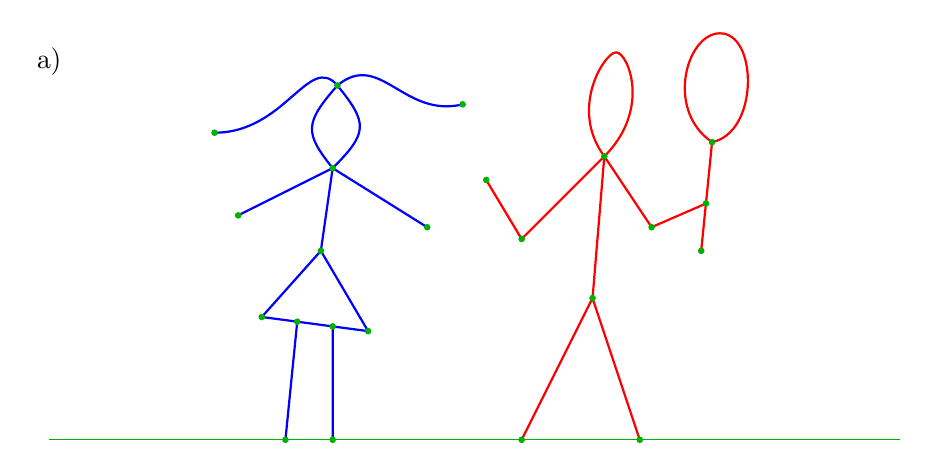
\begin{tikzpicture}[scale=0.6]
      \node at (0,8) {a)};
      \draw[green!70!black] (0,0) -- (18,0);
      \draw[blue,thick] (5,0) coordinate (b1) -- (5.25,2.5) coordinate (b2) -- (4.5,2.6) coordinate (b3)
      			-- (5.75,4) coordinate (b4) -- (6.75,2.3) coordinate (b5) -- (6,2.4) coordinate (b6)
			-- (6,0) coordinate (b7) (b2) -- (b6) (b4) -- (6,5.75) coordinate (b8) -- (8,4.5) coordinate (b9)
			(b8) -- (4,4.75) coordinate (b10) (b8) ..controls (6.75,6.5) and (6.75,6.7) .. (6.1,7.5) coordinate (b11)
			..controls (5.4,6.7) and (5.4,6.5) .. (b8) (b11) ..controls (7,8.25) and (7.5,6.8).. 
			(8.75,7.1) coordinate (b12) (b11) ..controls (5.5,8.2) and (5,6.5) .. (3.5,6.5) coordinate (b13);
      \draw[red,thick]  (10,0) coordinate (r1) -- (11.5,3) coordinate (r2) -- (12.5,0) coordinate (r3)
      			(r2) -- (11.75,6) coordinate (r4) -- (10,4.25) coordinate (r5) -- (9.25,5.5) coordinate (r6)
			(r4) -- (12.75,4.5) coordinate (r7) -- (13.9,5) coordinate (r8) -- (13.8,4) coordinate (r9)
			(r8) -- (14.03,6.3) coordinate (r10) ..controls (15,6.5) and (15,8.5) .. (14.26,8.6)
			..controls (13.52,8.7) and (13,7).. (r10)
			(r4) ..controls (12.75,7) and (12.25,8.2) .. (12,8.2) ..controls (11.75,8.2) and (11,7) .. (r4);
      \foreach\i in {1,...,13} { \fill[green!70!black] (b\i) circle (2pt); }
      \foreach\i in {1,...,10} { \fill[green!70!black] (r\i) circle (2pt); }
    \end{tikzpicture}

    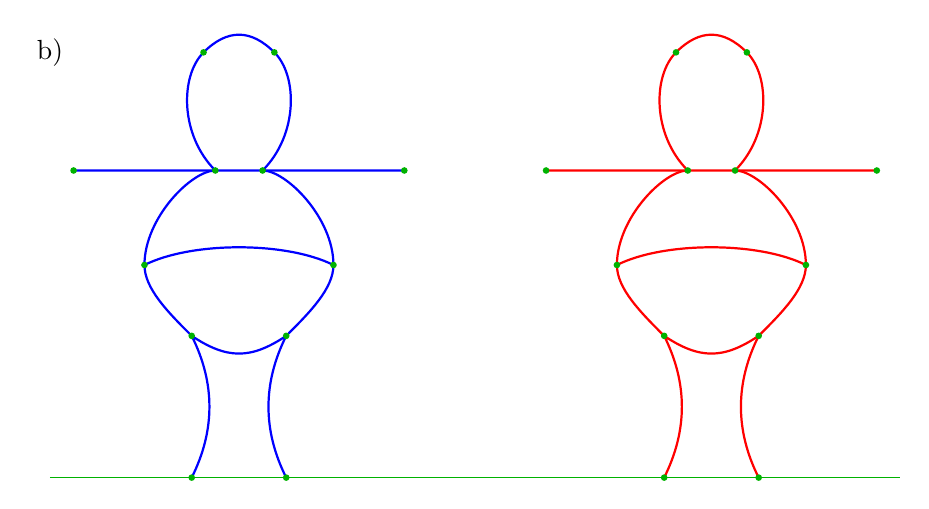
\begin{tikzpicture}[scale=0.6]
      \node at (0,9) {b)};
      \draw[green!70!black] (0,0) -- (18,0);
      \draw[blue,thick] (3,0) coordinate (b1) ..controls (3.5,1) and (3.5,2) .. (3,3) coordinate (b2)
      			..controls (3.75,2.5) and (4.25,2.5) .. (5,3) coordinate (r1)
			(2,4.5) coordinate (r3) ..controls (3,5) and (5,5) .. (6,4.5) coordinate (b3)
			..controls (6,4) and (5.5,3.5) .. (r1) (r3) ..controls (2,5.5) and (3,6.5) ..
			(3.5,6.5) coordinate (b4) -- (4.5,6.5) coordinate (r4)
			(b4) ..controls (2.75,7.25) and (2.75,8.5) .. (3.25,9) coordinate (b5)
			..controls (3.75,9.5) and (4.25,9.5) .. (4.75,9) coordinate (r5)
			(r4) -- (7.5,6.5) coordinate (b6);
      \draw[blue,thick]  (5,0) coordinate (r2) ..controls (4.5,1) and (4.5,2) .. (r1)
      			(b2)..controls (2.5,3.5) and (2,4) .. (r3)
			(r4) ..controls (5,6.5) and (6,5.5) .. (b3)
			(r5) ..controls (5.25,8.5) and (5.25,7.25) .. (r4)
			(b4) -- (0.5,6.5) coordinate (r6);
      \foreach\i in {1,...,6} {
        \fill[green!70!black] (b\i) circle (2pt);
        \fill[green!70!black] (r\i) circle (2pt);
      }

      \draw[red,thick,shift={(10,0)}] (3,0) coordinate (b1) ..controls (3.5,1) and (3.5,2) .. (3,3) coordinate (b2)
      			..controls (3.75,2.5) and (4.25,2.5) .. (5,3) coordinate (r1)
			(2,4.5) coordinate (r3) ..controls (3,5) and (5,5) .. (6,4.5) coordinate (b3)
			..controls (6,4) and (5.5,3.5) .. (r1) (r3) ..controls (2,5.5) and (3,6.5) ..
			(3.5,6.5) coordinate (b4) -- (4.5,6.5) coordinate (r4)
			(b4) ..controls (2.75,7.25) and (2.75,8.5) .. (3.25,9) coordinate (b5)
			..controls (3.75,9.5) and (4.25,9.5) .. (4.75,9) coordinate (r5)
			(r4) -- (7.5,6.5) coordinate (b6);
      \draw[red,thick,shift={(10,0)}]  (5,0) coordinate (r2) ..controls (4.5,1) and (4.5,2) .. (r1)
      			(b2)..controls (2.5,3.5) and (2,4) .. (r3)
			(r4) ..controls (5,6.5) and (6,5.5) .. (b3)
			(r5) ..controls (5.25,8.5) and (5.25,7.25) .. (r4)
			(b4) -- (0.5,6.5) coordinate (r6);
      \foreach\i in {1,...,6} {
        \fill[green!70!black] (b\i) circle (2pt);
        \fill[green!70!black] (r\i) circle (2pt);
      }
    \end{tikzpicture}

    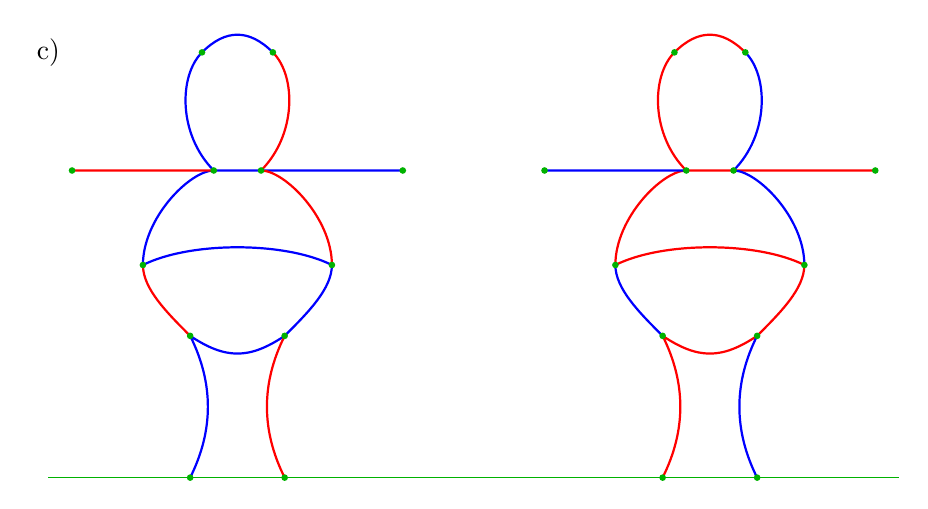
\begin{tikzpicture}[scale=0.6]
      \node at (0,9) {c)};
      \draw[green!70!black] (0,0) -- (18,0);
      \draw[blue,thick] (3,0) coordinate (b1) ..controls (3.5,1) and (3.5,2) .. (3,3) coordinate (b2)
      			..controls (3.75,2.5) and (4.25,2.5) .. (5,3) coordinate (r1)
			(2,4.5) coordinate (r3) ..controls (3,5) and (5,5) .. (6,4.5) coordinate (b3)
			..controls (6,4) and (5.5,3.5) .. (r1) (r3) ..controls (2,5.5) and (3,6.5) ..
			(3.5,6.5) coordinate (b4) -- (4.5,6.5) coordinate (r4)
			(b4) ..controls (2.75,7.25) and (2.75,8.5) .. (3.25,9) coordinate (b5)
			..controls (3.75,9.5) and (4.25,9.5) .. (4.75,9) coordinate (r5)
			(r4) -- (7.5,6.5) coordinate (b6);
      \draw[red,thick]  (5,0) coordinate (r2) ..controls (4.5,1) and (4.5,2) .. (r1)
      			(b2)..controls (2.5,3.5) and (2,4) .. (r3)
			(r4) ..controls (5,6.5) and (6,5.5) .. (b3)
			(r5) ..controls (5.25,8.5) and (5.25,7.25) .. (r4)
			(b4) -- (0.5,6.5) coordinate (r6);
      \foreach\i in {1,...,6} {
        \fill[green!70!black] (b\i) circle (2pt);
        \fill[green!70!black] (r\i) circle (2pt);
      }

      \draw[red,thick,shift={(10,0)}] (3,0) coordinate (b1) ..controls (3.5,1) and (3.5,2) .. (3,3) coordinate (b2)
      			..controls (3.75,2.5) and (4.25,2.5) .. (5,3) coordinate (r1)
			(2,4.5) coordinate (r3) ..controls (3,5) and (5,5) .. (6,4.5) coordinate (b3)
			..controls (6,4) and (5.5,3.5) .. (r1) (r3) ..controls (2,5.5) and (3,6.5) ..
			(3.5,6.5) coordinate (b4) -- (4.5,6.5) coordinate (r4)
			(b4) ..controls (2.75,7.25) and (2.75,8.5) .. (3.25,9) coordinate (b5)
			..controls (3.75,9.5) and (4.25,9.5) .. (4.75,9) coordinate (r5)
			(r4) -- (7.5,6.5) coordinate (b6);
      \draw[blue,thick,shift={(10,0)}]  (5,0) coordinate (r2) ..controls (4.5,1) and (4.5,2) .. (r1)
      			(b2)..controls (2.5,3.5) and (2,4) .. (r3)
			(r4) ..controls (5,6.5) and (6,5.5) .. (b3)
			(r5) ..controls (5.25,8.5) and (5.25,7.25) .. (r4)
			(b4) -- (0.5,6.5) coordinate (r6);
      \foreach\i in {1,...,6} {
        \fill[green!70!black] (b\i) circle (2pt);
        \fill[green!70!black] (r\i) circle (2pt);
      }
    \end{tikzpicture}
  \end{center}
\end{aufgabe}

In Bild a hat Blau 14 Züge und Rot 11 Züge, in denen sie ziehen können, wenn sie sich von oben nach unten auf ihrer Seite
vorarbeiten. Rot kann also nichts dagegen tun, dass Blau am Ende 3 Züge mehr hat. Diesen Vorteil von Blau können wir ausgleichen,
indem wir einfach drei rote Striche auf dem Boden hinzufügen: das so veränderte Spiel ist dann ein Nullspiel. Wir sagen, dass Blau
\emph{einen Vorteil von drei Zügen hat} oder dass das Spiel den Wert $-3$ hat. Hätte Rot den Vorteil, dann würden wir sagen, dass
das Spiel den Wert $+3$ hat. (Natürlich ist das Vorzeichen hier willkürlich gewählt: Wir könnten genauso gut sagen, dass ein
Vorteil für Rot einen negativen und ein Vorteil für Blau einen positiven Wert ergibt. Man muss sich nur auf eine Konvention
festlegen.)

Sowohl in Bild b als auch in Bild c kann der Spieler, der nicht beginnt, immer den Zug des jeweils anderen nachmachen und hat so
immer einen Zug, wenn der erste Spieler noch einen Zug übrig hat. Durch diese \emph{Nachäff-Strategie} gewinnt also jeweils
derjenige, der nicht beginnt, egal, wie gut der Beginnende spielt. Es handelt sich also hier um Nullspiele.

Doch nicht alle Spiele lassen sich durch ganze Züge auf dem Boden zu Nullspielen machen. Ein Beispiel dafür ist folgende
Situation:

\begin{center}
  \begin{tikzpicture}[scale=0.7]
    \draw[green!70!black] (0,0) -- (9,0);
    \draw[green!70!black,dashed] (4,-0.5) -- (4,2.5);
    \draw[blue,thick] (2,0) coordinate (b1) -- (2,1) coordinate (b2) (6,0) coordinate (b3) -- (6,1) coordinate (b4);
    \draw[red,thick]  (b2) -- (2,2) coordinate (r1) (b4) -- (6,2) coordinate (r2) (7,0) coordinate (r3) -- (7,1) coordinate (r4);
    \foreach\i in {1,...,4} {
      \fill[green!70!black] (b\i) circle (2pt);
      \fill[green!70!black] (r\i) circle (2pt);
    }
    \node at (2,-0.5) {A};
    \node at (6.5,-0.5) {B};
  \end{tikzpicture}
\end{center}

Bei Situation A ist Spieler Blau im Vorteil, denn egal ob Rot davor zieht oder nicht, kann Blau den einen Strich seiner Farbe
entfernen und es sind danach keine roten Steine mehr übrig. Ganz anders ist die Situation bei B: Wenn Blau beginnt, hat Rot immer
noch einen Strich seiner Farbe übrig, der entfernt werden kann, und wenn Rot beginnt, kann er einfach den Strich entfernen, der
auf dem blauen Strich sitzt, und gewinnt dann eine Runde später. Der Wert von B ist allerdings um 1 größer als der Wert von A, da
wir einen Strich für Rot auf dem Boden hinzugefügt haben, also einen Zug Vorteil für Rot.

Das bedeutet, dass der Wert von A irgendwo zwischen $-1$ und $0$ liegen muss. Doch was ist der genaue Wert von A? Dafür schauen
wir uns folgendes Spiel an:

\begin{center}
  \begin{tikzpicture}[scale=0.7]
    \draw[green!70!black] (0,0) -- (6,0);
    \draw[blue,thick] (2,0) coordinate (b1) -- (2,1) coordinate (b2) (3,0) coordinate (b3) -- (3,1) coordinate (b4);
    \draw[red,thick]  (b2) -- (2,2) coordinate (r1) (b4) -- (3,2) coordinate (r2) (4,0) coordinate (r3) -- (4,1) coordinate (r4);
    \foreach\i in {1,...,4} {
      \fill[green!70!black] (b\i) circle (2pt);
      \fill[green!70!black] (r\i) circle (2pt);
    }
    \node at (3,-0.5) {C};
  \end{tikzpicture}
\end{center}

Die Situation C ist zusammengesetzt aus zwei Mal A und einem Zug Vorteil für Rot, also ist der Wert von C gleich zweimal dem Wert
von A plus $1$. Allerdings kann man sich überlegen, dass C ein Nullspiel ist, indem man alle Möglichkeiten durchgeht: Wenn Rot
beginnt, kann er entweder den Strich ganz rechts wegnehmen: Dann sind nach den nächsten zwei Zügen von Blau auch die roten Striche
alle entfernt. Andererseits könnte Rot auch einen Strich, der auf einem blauen Strich steht, entfernen. In diesem Fall würde Blau
seinen anderen Strich (und damit den daraufstehenden roten Strich) wegnehmen und wieder gewinnen. Wenn aber Blau beginnt, entsteht
nach einem Zug die Situation B, die wir schon als Vorteil für Rot identifiziert haben. Also: Wenn Rot beginnt, gewinnt Blau, und
wenn Blau beginnt gewinnt Rot. Es handelt sich also um eine Nullposition.

Also ist der Wert von C gleich $0$ (kurz: $C=0$). Das war aber gleich zwei mal der Wert von A plus $1$ (kurz: $C=2\cdot A+1$).
Zweimal der Wert von A muss also $-1$ sein, das heißt, der Wert von A ist $-\frac 12$.
Blau hat also in Situation A einen halben Zug Vorteil. Die folgende Aufgabe zeigt, dass es auch Viertelzüge gibt:

\begin{aufgabe}\
  \begin{center}
    \begin{tikzpicture}[scale=0.7]
      \draw[green!70!black] (0,0) -- (15,0);
      \draw[green!70!black,dashed] (4,-0.5) -- (4,3.5) (9,-0.5) -- (9,3.5);
      \draw[blue,thick] (2,0) coordinate (b1) -- (2,1) coordinate (b2)
      	                (6,0) coordinate (b3) -- (6,1) coordinate (b4)
			(7,1) -- (7,2) coordinate (b5)
			(11,0) coordinate (b6) -- (11,1) coordinate (b7)
			(12,0) coordinate (b8) -- (12,1) coordinate (b9)
			(13,1) -- (13,2) coordinate (b10);
      \draw[red,thick]  (2,1) -- (2,2) coordinate (r1) -- (2,3) coordinate (r2)
      			(6,1) -- (6,2) coordinate (r3) -- (6,3) coordinate (r4)
			(7,0) coordinate (r5) -- (7,1) coordinate (r6)
			(11,1) -- (11,2) coordinate (r7) -- (11,3) coordinate (r8)
			(12,1) -- (12,2) coordinate (r9) -- (12,3) coordinate (r10)
			(13,0) coordinate (r11) -- (13,1) coordinate (r12);
      \foreach\i in {1,...,10} {
	\fill[green!70!black] (b\i) circle (2pt);
      }
      \foreach\i in {1,...,12} {
	\fill[green!70!black] (r\i) circle (2pt);
      }
      \node at (2,-0.5) {A};
      \node at (6.5,-0.5) {B};
      \node at (12,-0.5) {C};
    \end{tikzpicture}
  \end{center}

  Überlege dir, dass C ein Nullspiel ist. Was ist der Wert von A?
\end{aufgabe}

\end{document}
